\documentclass[sigconf]{acmart}

\usepackage[utf8]{inputenc}

%% For algorithms
\usepackage{algorithm}
\usepackage{algpseudocode}

%% For bibtex
\usepackage{natbib}

%% for good tables
\usepackage{array}
\usepackage{booktabs}

% \setlength{\parskip}{0.3em}

% Misc to use bépo keyboard.
\DeclareUnicodeCharacter{00A0}{~}
\DeclareUnicodeCharacter{00D7}{\times}

% Helper commands
\newcommand{\tl}{\textless}
\newcommand{\tg}{\textgreater}

\newcommand{\bb}[1]{\mathbb{#1}} % the blackboard bold capital is used for sets.



\setcopyright{rightsretained}

% DOI
\acmDOI{10.1145/nnnnnnn.nnnnnnn}

% ISBN
\acmISBN{978-x-xxxx-xxxx-x/YY/MM}

% Conference
\acmConference[GECCO '18]{the Genetic and Evolutionary Computation
Conference 2018}{July 15--19, 2018}{Kyoto, Japan}
\acmYear{2018}
\copyrightyear{2018}

\acmPrice{15.00}

\acmSubmissionID{123-A12-B3}

\begin{document}

\title{Humane approach to Starcraft micromanagement}

\author{Benoît Cortier}
\affiliation{\institution{University of Technology of Belfort-Montbéliard}
             \streetaddress{90010 cedex}
             \city{Belfort}
             \country{France}
             }
\affiliation{\institution{University of Tsukuba, Graduate School of Systems and Information Engineering}
             \streetaddress{Tennodai 1-1-1}
             \city{Tsukuba City}
             \country{Japan}
             }
\email{benoit.cortier@fried-world.eu}

\author{Claus Aranha}
\affiliation{\institution{University of Tsukuba, Faculty of Engineering, Information and Systems}
             \streetaddress{Tennodai 1-1-1}
             \city{Tsukuba City}
             \country{Japan}
             }
\email{caranha@cs.tsukuba.ac.jp}

% 174 words (Maximum 200 words)
\begin{abstract}
We study the use of NEAT and variants to develop strategies for the
micromanagement of squads of units in the Starcraft: Brood Wars game.
While current research in this field focuses on developing strategies
that maximize win rate, we are interested in also minimizing the amount
of losses in terms of destroyed units. This is important when one considers
that Starcraft battles are in the context of a longer strategic play session,
and in this sense conserving resources is important. To achieve this goal,
we defined a fitness function that takes into account the number of
surviving units, and experimented with four NEAT variants: vanilla NEAT,
Novelty Search applied to NEAT, unified (or homogeneous) NEAT and Cascade-NEAT. We
explored these four variants on with four different units matchups. The
four variants performed similarly on win ratio and survival metrics.
However, we performed a qualitative analysis as well and found that differents
behaviours emerged or that they emerged in different ways. From all that we draw
ideas for future work that could achieve our original goal.
\end{abstract}

\begin{CCSXML}
<ccs2012>
<concept>
<concept_id>10010405.10010476.10011187.10011190</concept_id>
<concept_desc>Applied computing~Computer games</concept_desc>
<concept_significance>500</concept_significance>
</concept>
</ccs2012>
\end{CCSXML}

\ccsdesc[500]{Applied computing~Computer games}

\keywords{Starcraft, micromanagement, NEAT, neuroevolution, artificial
          neural networks, evolutionary algorithms, RTS}

\maketitle

\section{Introduction}\label{section:introduction}

\emph{Starcraft: Brood Wars} is a Real Time Strategy (RTS) computer
game that has in recent years captured the attention of researchers on
game-playing artificial intelligence. StarCraft is a complex game that
can be studied from many different points of view: Strategic Planning,
Execution of tactical manuevers, Estimation of hidden information
about the opponent, etc.

In this work, we focus on the problem of ``micro'' in
Starcraft. Micro, short for micromanagement, is the problem of
directly controlling a small number of units directly in an engagement
with units from an opponent player. The tasks required in micro
include moving damaged units out of the fire range from the enemy,
spreading the units to maximize the fire arc, and using an unit's
special abilities at the right time. Also, the decisions for each of
these tasks will differ according to the units controlled by the
player and the opponent.

Micro has been studied by many groups recently, such as {\bf TODO,
  include some papers and their tools here}.

In these studies, a successful micro technique is usually measured by
the ``win rate'', defined as the percentage of pre-defined encounters
where all the enemy units have been destroyed by the player
units. However, in an actual game, being able to preserve your own
units can be as important as being able to defeat the enemy
units. Therefore, in this study we {\bf TODO...}




\section{Background}\label{section:background}

\subsection{Starcraft}

Starcraft is a \emph{Real Time Strategy} (RTS) game published by
Blizzard Entertainment. It follows the ``gather-build-conquer''
pattern, in which each player (human or AI) must gather resources
available in the play field to build combat units and
structures. These units are used to attack the other players,
destroying their units and structures and denying their access to
resources. The game features a wide variety of combat units, with
different speeds, attack range, strengths and weakenesses. The balance
between combat and resource gathering leads to the concepts of
\emph{micromanagement} (micro) and \emph{macromanagement}
(macro). Micro are the tactical actions and skills involving
individual battles between a game, while Macro are the strategic
decisions such as building management, resource usage, and unit
creation. A successful player (or bot) needs to eventually master
these two aspects of the game.

Development of AI agents for Starcraft is a vibrant research field
(See surveys by Onta\~non~\cite{Ontanon13AICompetitionSurvey} and
Certicky~\cite{Certicky17SurveyCompetitionsBots}). They highlight that, unlike Go and Chess,
Starcraft presents Game Playing AI the challenge of dealing with
real-time, partial information scenarios. Therefore, Starcraft is a
hard challenge for AI. An unofficial framework for the development of
AI agents exists in the form of the \emph{Brood Wars API}
(BWAPI)~\cite{BWAPI}. It allows the user to read and write to the
game's memory, allowing a wide range of agent types, from agents that
control limited parts of an AI opponent, to agents with the same range
of inputs and outputs as a human player.

% This requires good thinking, decision making and fast reactions.
% The game features three different races and all units are unique to
% their respective races, performs differently and requires different
% tactics.  The game is well known for being well balanced and as such
% was widely used in competitions.  Indeed even though each race is
% unique, has different strengths and abilities, their overall
% strength is the same and no race has an advantage over the
% other. This is because the game is now quite old and the balance
% have been polished over time via game updates provided by Blizzard
% Entertainment, developer and publisher of the game. It makes this
% game a great support to develop competitive, modular, adaptative
% agents.

% To create Starcraft: Broodwar agents, the \emph{BWAPI (Brood War
% Application Programming Interface) free and open source C++
% framework} is widely used by students, researchers and
% hobbyists. This framework isn't an official product from Blizzard
% and access and modify the game state by reading and writing directly
% the memory space of the game. As such is considered to be a "hack"
% that violates the End User License Agreement of the game. However,
% it is tolatered by company (and even encouraged given that they
% provided prizes to the tournament sponsorised by
% AIIDE\footnote{Artificial Intelligence and Interactive Digital
% Entertainment}). Reading / writing directly in the memory space of
% another program is considered to be an unsafe method (at least in
% term of stability) but the framework has been used and maintained
% for a long time and is considered stable.  It can be configured so
% as to only reveals the parts of the game state that are visibles by
% the agent, effectively providing only information that a real human
% player would have access to. That way, it is possible to write
% non-cheating AIs that operate under partial information conditions.

\subsection{Micromanagement}

In this study we focus on the \emph{Micromanagement} (Micro) aspect of
an Starcraft controller. Micro refers to the control of individual
units involved in a tactical combat. This involves sending commands to
each individual unit as a player would do, such as ``attack unit A'' or
``move to position X,Y''.


There are many approaches to developing Starcraft micro
controllers. Wender and Watson investigate the viability of
Reinforcement Learning to this task~\cite{Wender12ReinforcementMicroSC}. They show that a
variety of RL techniques could achieve 100\% win ratios in small
combat situations, by controlling two actions: ``Attack'' and
``Retreat''.

Shantia et al. explore the use of neural networks to also order a unit
to ``attack'' or ``flee''~\cite{Shantia11ConnectionistSC}. The weights of the neural
network are adjusted by a RL algorithm. They show that you can train
the neural network on smaller combats (3x3) to perform well in larger
engagements (6x6).

More recently, Neuro Evolution has become a popular approach for
training Starcraft controllers. Zhen and Watson show a comparison of
NEAT and rtNEAT~\cite{Zhen13NeuroEvoSC} for training a micro controller (also
using ``Attack'' and ``Retreat''). Their setup includes four classes
of engagement (ranged vs melee, melee vs melee, ranged vs ranged and
melee vs ranged), each with two teams of 12 units. They remark how the
unit composition of the matchup has an effect on the variability of
the result.

One thing that all of these approaches (and a few others) have in
common is that the evaluation of the training is based on the win
ratio and the number of enemies killed. In this study, we want to
explore how to achieve a more ``humane'' behaviour, i.e. achieving
victories while at the same time conserving the fighting force and
maximizing the number of surviving units.

\subsection{NEAT}\label{subsec:neat}

NEAT (\emph{Neuro Evolution of Augmented Topologies}) is a machine
learning technique which combines neural network and evolutionary
computation ideas to develop both the weights and the topology
(structure) of a neural network~\cite{Stanley02Neat}.

NEAT begins with a minimal topology, and grows it through training in
order to match the problem difficulty, adding and removing neurons and
connections and changing weights. Self connections and connections to
different layers are possible, which means that NEAT can evolve
recurrent neural networks. Additionally, NEAT includes a speciation
mechanism to promote genetic diversity in the population.

rtNEAT is a variant of NEAT for real time problems, which was
originally demonstrated on the combat game NERO. Since then, NEAT and
rtNEAT have been popular choices for the training of controllers in
tactical scenarios. The ability to match each unit to a separate
network in the population, and the ability to progressively learn more
complex behaviours are two compelling reasons for the use of
NEAT/rtNEAT in Starcraft.

Accordingly, recently variants of NEAT such as Cascade-NEAT have also
been proposed to answer to specific problems.

\subsection{Cascade-NEAT}\label{subsec:cascade-neat}

Cascade-NEAT is a variant of NEAT which aims at restricting the neural
network search space to topologies that have a so-called cascade
architecture. A cascade architecture means that all hiden neurons are
connected to all other neurons, and only connections associated with
the most recently added hidden neuron are modified by the evolutionary
process.

Kohl~\cite{Kohl09FracturedProblems, Kohl09StrategicDecisions} reports that this method is good for
fractured problems, such as the concentric spiral clustering problem
and the keepaway soccer decision problem. However, Cascade-NEAT
performs very poorly on some problems requiring recurrent connectivity
patterns, since it cannot produce such patterns. An example of such
failure is the non-Markovian double pole-balancing problem for which
Cascade-NEAT doesn't find a single suitable solution whereas the
standard NEAT performs very well.

To our knowledge, Cascade-NEAT has not been applied to the Starcraft
problem. Because of the similarity of some strategic decisions
involved in Starcraft micro management and the keepaway soccer problem
we decided to include Cascade-NEAT as one of the alternatives for the
current investigation.

\subsection{Novelty search}\label{subsec:novelty-search}

Novelty search is a new approach to planning and search algorithms
where, instead of rewarding the agents for progressing towards a fixed
objective, agents are rewarded for finding solutions that are different
from other solutions already found by the algorithm.

Surprisingly, sometimes not explicitly looking for the objective leads
to finding a solution faster, specially in the case of deceptive
problems.  Indeed, intermediate steps and partial solutions may
require an evolution towards a completely different direction than
that of the final expected result. In these cases, objective-oriented
algorithms may get stuck in local optima and cause the search to
fail.

\citet{Lehman11Novelty} demonstrated this with an experiment where a
robot controlled by a neural network has to find a specific location
in a maze. A solution's Novelty is characterized by the end location
of the robot, compared to all others so far. Only Novelty Search was
able to find the goal in the deceptive maze.

\subsection{Potential fields}\label{subsec:potential-fields}

Potential Fields, also called Artificial Potential Fields (APF), is a
method using the idea of attracting and repelling fields in a
space. It is mainly used for planning tasks involving maneuvering.
The sum of all the fields given the agent's position is used to
determine the direction for its next move. The strength of a
particular field on the agent's movement is proportional to the
closeness of that agent to the field's center

This algorithm was originally used to make robots navigate between
obstacles. Obstacles are given a repelling fields while the objective
is given an attractive field. However, using it in RTS games has been
explored as well \cite{Hagelback08RTSPotentialFields}.
\citet{Svendsen12SCPotentialFieldsGP} applied this method to
StarCraft micromanagement along with a multi-objective evolutionary
algorithm called NSGA-II to optimize the fields automatically.



\section{Proposal}\label{section:proposal}

A fresh C++ implementation of these methods was developed and is
hosted on Github under the name of LIBRARY
NAME\footnote{\url{https://github.com/uuuuu/nnnnn}}.%NEToolKit\footnote{\url{https://github.com/CBenoit/NEToolKit}}.

The Starcraft bot can be found on Github as well under the name of BOT
NAME\footnote{\url{https://github.com/uuuuu/nnnnn}}.%Evolubot\footnote{\url{https://github.com/CBenoit/Evolubot}}.

The analysis of the data was performed with the R language. Sources
can, again, be found on
Github\footnote{\url{https://github.com/uuuuu/nnnnn}}.%\footnote{\url{https://github.com/CBenoit/EvolubotAnalysis}}.

We want to evaluate several techniques that are the following:
\begin{itemize}
    \item \emph{Vanilla NEAT}. The default NEAT, as described in
      Sub-Section~\ref{subsec:neat}. One generation is evaluated with
      one game where every unit is an individual with its own neural
      network. Therefore, the fitness is individual on a per unit
      basis.
    \item \emph{Cascade-NEAT}. The cascade-NEAT variant, as described
      in Sub-Section~\ref{subsec:cascade-neat}.  The evaluation mothed
      is the same as for vanilla NEAT above.
    \item \emph{Novelty Search with vanilla NEAT}. The novelty search
      method as described in Sub-Section~\ref{subsec:novelty-search}
      applied to the NEAT algorithm.  The evaluation methed is the
      same as for vanilla NEAT above.
    \item \emph{``Unified'' networks with vanilla NEAT}. For this one,
      as opposed to the evaluation method explained above, only one
      indivual is evaluated per game and thus to evaluate a whole
      generation, a number of games equal to the population size must
      be processed.  The fitness of an indivual is computed by how
      well all the controlled units performs. Each unit still has its
      own neural network but, they're all obtained by using the genome
      of the individual being evualated.
\end{itemize}

We consider that in an actual game, being able to preserve one's units
can be as important as being able to defeat the enemy units.
Therefore, in this study we will measure survival rates as well.

\subsection{Neural Networks Inputs and Outputs}

For all the matchups, we will generate networks with at least the
following inputs:
\begin{itemize}
    \item The \emph{cooldown} of the ground weapon.
    \item The \emph{distance} to the \emph{closest enemy}.
    \item The \emph{number} of enemies \emph{in sight}.
    \item The \emph{distance} to the \emph{closest allies}.
    \item The \emph{number} of allies \emph{in sight}.
\end{itemize}

And the following outputs:
\begin{itemize}
    \item \emph{Attack} the \emph{weakest enemy in fire range}.
    \item \emph{Retreat} from the battlefield: \emph{draw away from enemies in sight}.
    \item \emph{Spread out}: \emph{draw away from allies in sight}.
    \item \emph{Gathering}: get close to \emph{allies in sight}.
\end{itemize}

The \emph{attack} action consist of going in the direction of the closest enemy not in fog of war
and if there are severeral enemies in fire range, attack the weakest one.

As for \emph{retreat, spread out and gathering} actions, a weighted vector is computed
to lead the agent in a sensible way. This has been used by~\cite{Shantia11ConnectionistSC, Wender12ReinforcementMicroSC, Zhen13NeuroEvoSC} as well.
Our version differ slightly though. For retreat and spread out, it means for the agent to
get away from other units (enemies and allies) as fast as possible. The repulsive force's strength of an unit to
get away from is calculated by its proximity with the agent so that the more the unit is close,
the more urgent it is to get away from it specifically. For the retreat action, ally units
get a significantly smaller weight than enemy's ones so that the agent avoid collision with
allies while drawing away from enemies.
In case of the gathering action, attractive force is given to allies only.

In addition, marines get one additional input and output:
\emph{whether it is stimmed or not} as the input and \emph{use a
  stimpack} as the output.

\subsection{Fitness Specification}

The weights are used to model the fitness function. There are two
fitness functions, according to whether the Unified NEAT variant is
being used or not.  The regular fitness function is given by
\begin{equation*}
  (\text{damages\_dealt} \times A + \text{health} \times B + \text{survivors} \times C)^D,
\end{equation*}
while the fitness for the Unified NEAT variant is
\begin{equation*}
  (\text{damages\_dealt} \times A + \text{survivors} \times C)^D.
\end{equation*}
Here \emph{A} is the attack performance weight, \emph{B} the survival
performance weight, C is the cooperative performance weight and D is
the exponent on the fitness.

To encourage the variants to find strategies that promote cooperation
and survival, we have included the number of survivors as a component
of the fitness function.

Novelty currently just use fitness as novelty metrics which is not
the best use case at all for this method.



\section{Experiment Design}

We designed the following experiment to compare the four NEAT
implementations described in the previous session in regards to their
victory ratio and survival ratio.

\subsection{Match Specification}

The experiment focuses on a matchup between a squad of units
controlled by the NEAT implementation, and a squad of units controlled
by the standard starcraft controller. Four unit matchups were defined:
\begin{enumerate}
    \item 22 marines vs 22 marines
    \item 22 marines vs 44 zerglings
    \item 22 vultures vs 22 vultures
    \item 22 vultures vs 22 zealots
\end{enumerate}

\begin{figure}
    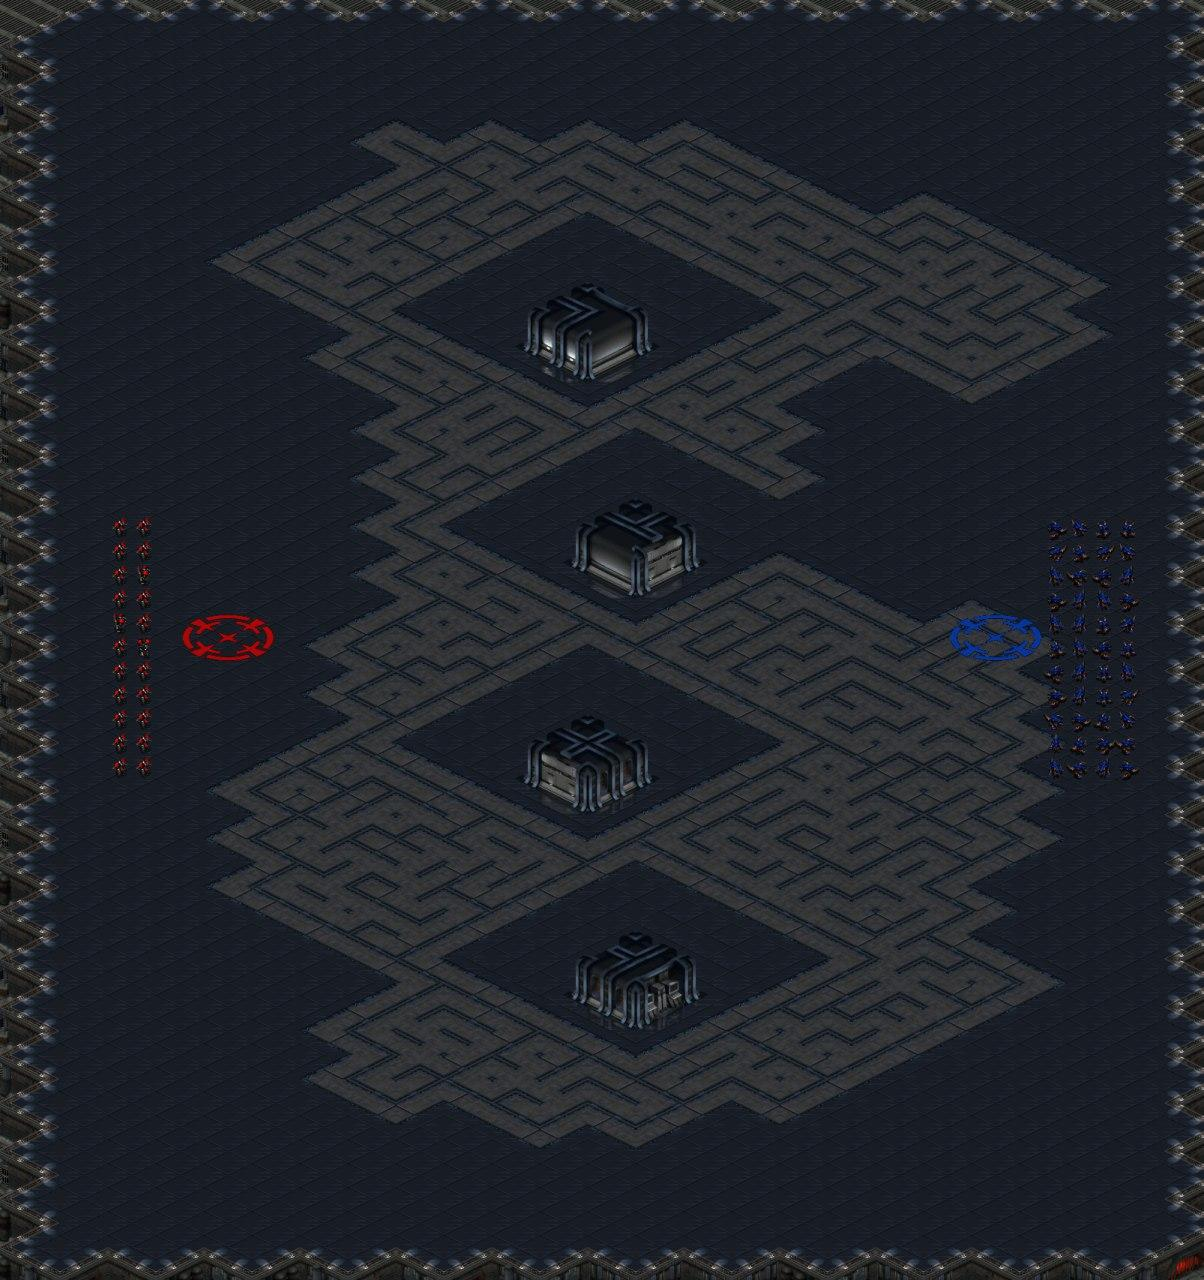
\includegraphics[width=.5\textwidth]{figures/scenario_map_overview}
    \caption{The map used for all matchups}\label{fig:map_overview}
\end{figure}

In these matchups, the marines have stimpacks, but no other upgrades
are added to the units. The match occurs in a custom map with four small obstacles
on the middle, and the units of both sides start at
opposite ends of the map as shown on Figure~\ref{fig:map_overview}.

The units matchup were chosen to see if the controller could learn a
kiting behavior that helps preserve units. Additionally, the case of
marines (matchups 1 and 2) has the additional problem of stimpack
usage: Using a stimpack damages the unit in exchange of a boost in
speed. This causes a deceptive problem where the usage of stimpack
causes a short term penalty in exchange of a possible longer term gain
in victory and survival ratios. In particular, the marine vs zerglings
matchup is very difficult to win without proper stimpack usage, so we
would expect the controllers to learn it.

\subsection{Learning and Comparison specification}

The comparison among techniques is composed of two stages: learning
and evaluation.

At the learning stage, we execute a complete evolution run with 100
generations for each combination of matchup and technique 3 times (for
a total of 48 evolution runs). The average fitness, best fitness and
number of survivors is logged for each generation.

After the learning stage, we evaluate each method by extracting the
five best genomes produced during the three evolution runs, and using
them for 50 games on an identical matchup. For these games, we log
the number of survivors and whether the game ended in victory or loss.

\subsection{Parameter Specifications}

Both the NEAT variants and the Starcraft Bot require multiple
parameters to be tuned in advance of any sort of experimentation. We
highlight some parameters that we feel are important for a better
understanding of the experimental results. A full list of the
parameters used can be obtained at the project github repository
listed in section~\ref{section:proposal}.

% IMPORTANT QUESTION: ARE WE USING A STANDARD NEAT LIBRARY? IF NOT,
% WHERE DO THE STANDARD NEAT PARAMETERS COME FROM?

\begin{tabular}{rll}
    \toprule
    Parameter & Value & Tweaks \\
    \midrule
    Number of inputs & 5 & 6 for marines \\
    Number of outputs & 4 & 5 for marines \\
    Initial population size & 22  & — \\[1ex]

    Compatibility threshold & 2 & — \\
    Dynamic compat. thresh. & true & — \\
    Target number of species & 4 & — \\
    Keep same species' representant & true & — \\[1ex]

    Use best genomes library & true & false if NS \\
    Bad genome max fitness & 100 & 1000 if Unified \\
    \bottomrule
\end{tabular}

The reason for overriding these parameters is as follows: The
\emph{initial population size} matches the number of controlled units
in the squad.  The \emph{number of inputs and outputs} for marines is
greater because the marine unit has to decide whether to use the
stimpack (output), and can sense whether the stimpack is ready for
activation (input). The \emph{keep same species' representant}
parameter is used to avoid the update of the representant of species
with a random member at each generation as described in the original
NEAT paper and instead keep the first representant of the species. The
best genomes library is not used for Novelty Search because NS does
not use the fitness as a performance metric. Instead, a separate list
of the best genomes is managed. The \emph{bad genome max fitness}
determine which genomes are to be considered bad given the
fitness. These genomes may occasionally be replaced by one from the
best genome library.

%The distance coefficients are used in the compatibility distance formula which is
%\[dist = c1 × \frac{E}{N} + c2 × \frac{D}{N} + c3 × W\]
%with N the number of genes of the larger genome, E the number of excess genes,
%D the number of disjoint genes and W the average weight differences of matching genes.
%The is the original compatibility distance formula.~\cite{Stanley02Neat}

Also, for the Cascade Neat variant, some mutation probabilities are modified:

\begin{tabular}{rl}
    \toprule
    Parameter & Value \\
    \midrule
    Add link & 0.00 \\
    Add neuron & 0.00 \\
    Remove neuron & 0.00 \\
    Add cascade & 0.03 \\
    Remove gene & 0.00 \\
    \bottomrule
\end{tabular}

These parameters were mostly taken from existing literature, that is the
original NEAT paper \cite{Stanley02Neat} and \cite{Kohl09FracturedProblems}.

%%%%%%%%%%%%%%%%%%%%%%%%%%%%%%%%%%%%%%%%%%%%%%%%%%%%%%%%%%%%%%%%%%%%%%%%%%%%

Finally, we discuss the parameters for the NEAT starcraft bot:

\begin{tabular}{rl}
    \toprule
    Parameter & Value \\
    \midrule
    Frames per update & 10 \\
    Max distance NN & 1500 \\
    Max entities NN  & 20 \\[1ex]

    Survival perf weight & 0.5 \\
    Attack perf weight  & 0.5 \\
    Cooperative perf weight & 10 \\
    Unified attack perf weight & 0.33 \\
    Unified cooperative perf weight & 100 \\
    Exponent on fitness & 1.3 \\
    \bottomrule
\end{tabular}

``Max distance NN'' and ``Max entities NN'' are, respectively, the
maximal distance and the maximal number of entities a neural network
can perceive.  This is used for normalization purposes. All values
greater than these will result in the value \(1\) being fed as the
input so that all inputs are in range \([0, 1]\).



\section{Experimental Results}\label{section:experiments-results}

\subsection{Quantitative Results}\label{subsec:quantitative}

As discussed in the previous session, the four NEAT variants were
compared in two ways: First we perform three full evolution runs for
each variant/matchup pairing, and then the five best genomes obtained
from this training are run 50 times to evaluate their victory and
survival ratios. A summary of these results is presented in
Table~\ref{table:quantitative}.

\begin{table}
    \caption{Victory Ratio and Median Survival for the best genomes.
            Survival values only consider victory matches.}
    \label{table:quantitative}
    \begin{tabular}{llll}
        \toprule
        Variant & Matchup & Win Ratio & Survival \\
        \midrule
        Vanilla & marine/marine & 0.77 & 8 \\
        Unified & marine/marine & 0.77 & 8 \\
        Cascade & marine/marine & 0.85 & 8 \\
        Novelty & marine/marine & 0.55 & 8 \\[1ex]

        Vanilla & marine/zergling & 0.03 & 4 \\
        Unified & marine/zergling & 0.01 & 10 \\
        Cascade & marine/zergling & 0.05 & 5 \\
        Novelty & marine/zergling & 0.09 & 10 \\[1ex]

        Vanilla & vulture/vulture & 0.92 & 8 \\
        Unified & vulture/vulture & 0.90 & 10 \\
        Cascade & vulture/vulture & 0.93 & 8 \\
        Novelty & vulture/vulture & 0.93 & 9 \\[1ex]

        Vanilla & vulture/zealot & 0.87 & 8 \\
        Unified & vulture/zealot & 0.93 & 9 \\
        Cascade & vulture/zealot & 0.92 & 9 \\
        Novelty & vulture/zealot & 0.99 & 9 \\
        \bottomrule
    \end{tabular}
\end{table}

% \subsubsection{Victory Rate Analysis}

From this table, we can observe that in general the methods managed to
learn a good tactic to defeat their enemies, with the exception of the
marine/zergling matchup.
%\footnote{This could be considered scientific evidence that Blizzard needs to nerf zerglings}
Small variations are observed on the methods within each matchup, but
an ANOVA test confirms that these variations are not significative (F
= 0.85).

% \subsubsection{Survival Rate Analysis}

In the same fashion, it was not possible to observe a clear difference
among the variants in terms of the median number of survivors in
winning matches. Figure~\ref{fig:survivors} shows the survivor numbers
for each variation/matching pairing.

\begin{figure}
  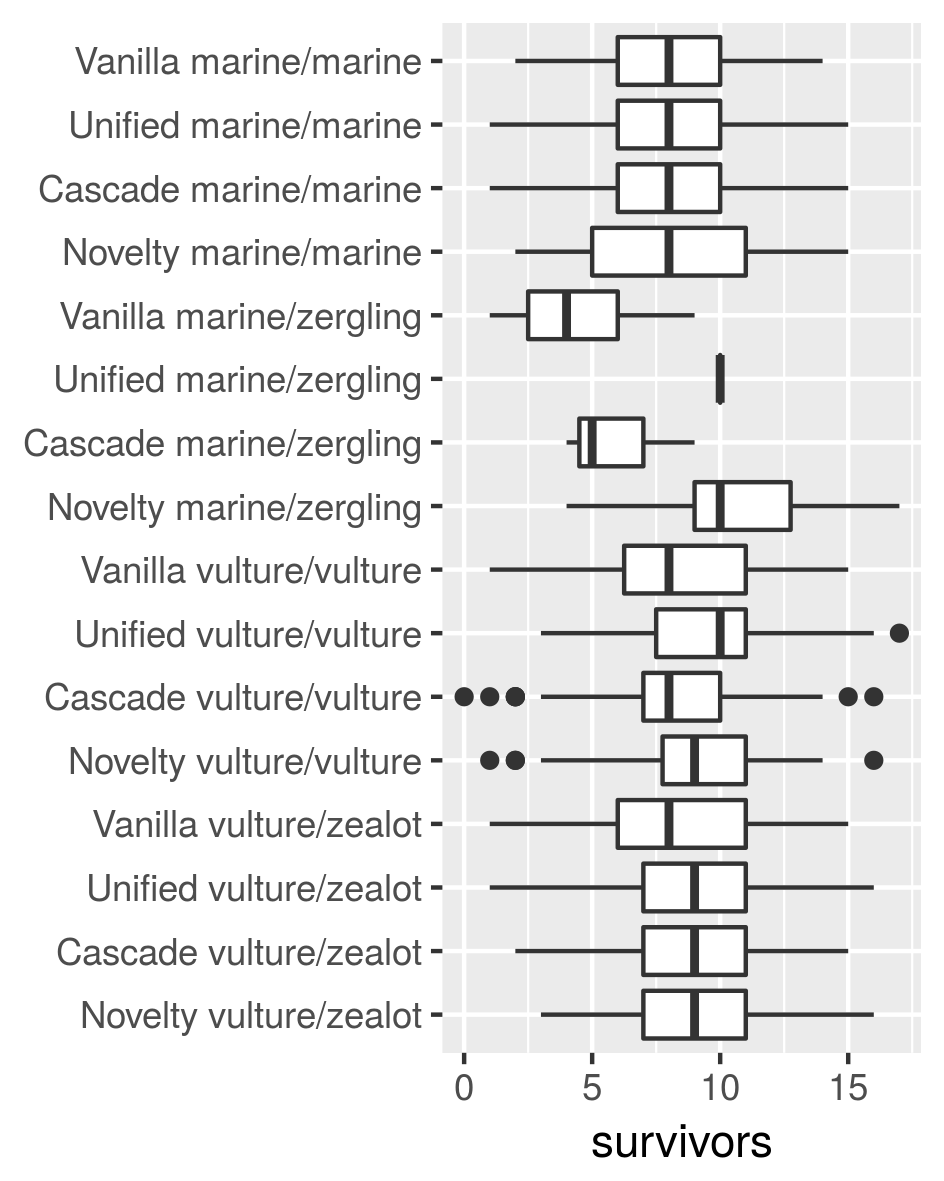
\includegraphics[width=.5\textwidth]{figures/survivors}
  \caption{Box plot for the survival ratios}\label{fig:survivors}
\end{figure}

% \subsubsection{Evolution Rate Analysis}


\begin{figure*}
  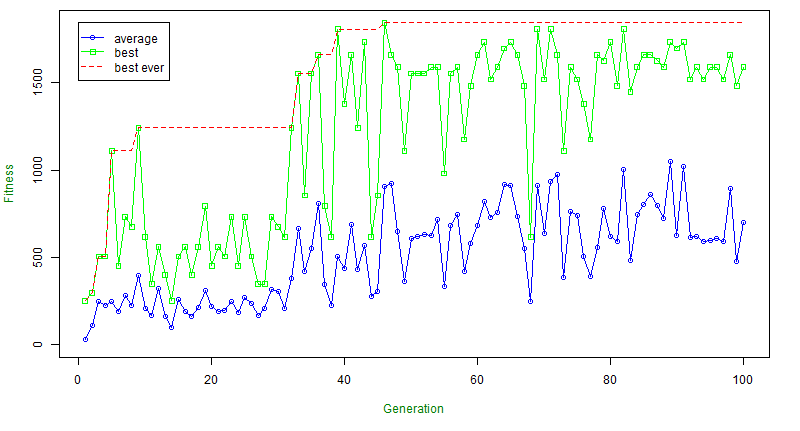
\includegraphics[width=.4\textwidth]{figures/evolution_zealot}
  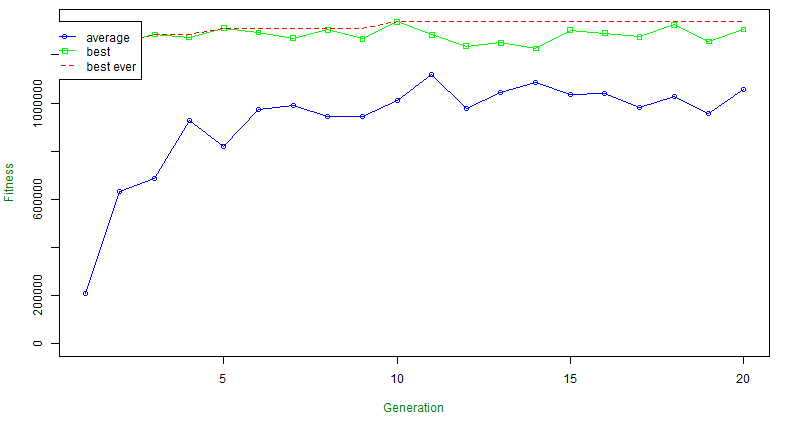
\includegraphics[width=.4\textwidth]{figures/evolution_unified}
  \caption{Training progress for two vulture vs zealot matchups. Left:
    Cascade-NEAT vs zealots. Right: Unified NEAT. Note that the
    fitness function are different so absolute values should not be
    compared directly.}\label{fig:evolution}
\end{figure*}

Finally, we observed the training progress of the
experiment. Figure~\ref{fig:evolution} show two examples of training
graphs that are representative of the experiment as a
whole\footnote{the figures for all matchings can be found at the
online repository}. In the Cascade-NEAT training (left side) we see
that while there is a small increase in best and mean fitness, there
are large variations every generation. In the Unified NEAT training
(right side) these variations are not present. In unified neat, all
networks in the same combat experiment share the same fitness result,
while in the other variants (such as the Cascade-NEAT) each network in
the same combat is evaluated separately, even though they influence
each other (a weak network will make the overall combat harder for a
stronger network).

However, while this difference is observable in the training curve, as
we see in Figure~\ref{fig:evolution}, it did not generate an
observable difference in the final result
(Table~\ref{table:quantitative}), which is interesting.

\subsection{Qualitative analysis}\label{subsec:qualitative}

From the quantitative analysis we learned that a winning strategy was
generally found (high winning ratio), while the differences among
variants was not strong. In particular, the survivor rate was the same
across methods with the exception of the particularly hard
marine/zergling matchup.

To better understand this lack of difference, and what could be done
to increase the survival ratio, we performed a qualitative analysis of the
results of the experiment by studying the different behaviours that emerged.

\subsubsection{Developping stimpack behaviour}

\begin{figure}
    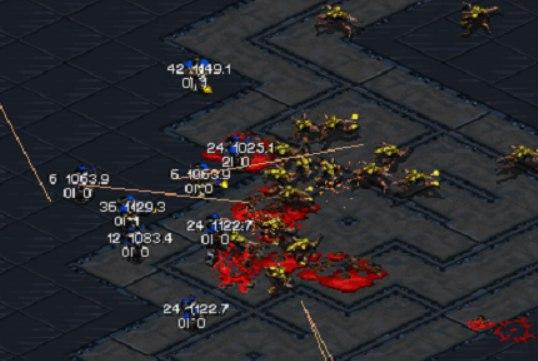
\includegraphics[width=.45\textwidth]{figures/marines_vs_zerglings_combat}
    \caption{Marines/Zerglings matchup. The Zergling speed makes this
      a hard matchup to win without stimpack
      behaviour}\label{fig:marines_vs_zerglings}
\end{figure}

The Marine/Zergling matchup was the hardest one of the four studied,
and the one where none of the NEAT variants managed to consistently
find a good solution. This is because the high speed of the zerglings
prevent the marines from develop a kiting behaviour
(Figure~\ref{fig:marines_vs_zerglings}).

To solve this problem, an agent needs to develop a \emph{stimpack
  behaviour}. Stimpack is an ability that increases the speed of the
marine for a few seconds, in exchange of an amount of its health. 

Vanilla NEAT and Cascade-NEAT didn't do a good job at developing this
stimpack behaviour. What we observed is that in a population where some
individuals use stimpack and some don't, the individuals that do not
use stimpack get better reward (because of their health), even though
their survival is because of the 'sacrifice' of the stimpack using
individuals, who rushed to the frontline and got themselves killed
first. The final result is that the stimpack behaviour gets lost over
the generations.

In comparison, the Unified Variant was somewhat better at developing
the stimpack behaviour. Since all agents in one combat use the same
genotype and have the same genotype, all of them are rewarded equally
for the use of stimpack, even if some units are lost early.

As for the Novelty Variant, the behaviour is lost less easily, and some
of the best genomes still use it. However, there is still a degree
of loss during the evolution, specially when some units in combat develop
a fleeing behaviour. However, the Novelty aspect might be just enough to
keep the less rewarded stimpack users in the gene pool, and help explain the
better result of Novelty search noticed in the previous section.

Overall, another reason for losing the stimpack behaviour is the timing
of its development during the training. If the fighting behaviour is
poor (for instance, not attacking the enemy or fleeing without
reason), stimpack usage will exarcebate the problem. We imagine that
it might be possible to develop a good stimpack behaviour with a better
Novelty measurement that does not use the fitness and more
appropriately model the Novelty of combat behaviours.

Additionaly, the marines vs marines matchup is solved differently from
the zergling matchup. We observed that in most cases this matchup can
be won by just waiting for the enemy and attacking all at once without
stimpack, which was precisely the convergent behaviour. This happens
because the initial enemy formation may lead to a line to form during
their advance, meaning that if the squad holds its original position
it can pick the enemy forces a part at a time, shooting first with
more firepower.

\subsubsection{Kiting behaviour}

\begin{figure}
    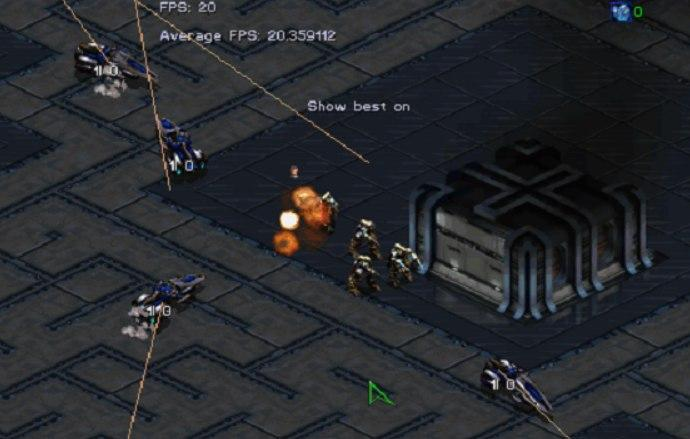
\includegraphics[width=.45\textwidth]{figures/vultures_kiting_screenshot}
    \caption{Vultures using kiting technique to beat
      zealots}\label{fig:vultures_kiting}
\end{figure}

All the studied variants performed exceedingly well on the
vulture/zealot matchup, as described in
section~\ref{subsec:quantitative}. This matchup illustrates the
\emph{kiting behaviour}, where a faster, long ranged unit has to keep a
distance from a short ranged opponent.

After a short number of generations, adequate individuals start to
emerge, even with the first species, meaning the topology required
isn’t complex at all. After a few more generations, networks weights
are tweaked to get a quite decent kiting behaviour for any variant.
The vulture is able to maintain a good distance between itself and the
enemies as shown on Figure~\ref{fig:vultures_kiting}. In some cases,
vultures are even able to shoot without losing speed and thus withdraw
really quickly from risks. This ressemble a classical vulture micro
technique called “patrol micro” involving the use of the so-called
patrol command's lack of cooldown to have the vulture move, fire, and
retreat without slowing down. We don’t really know how it is achieved
here without the patrol command, but it is effectively the same
result.

It is interesting to note that for the matchup vultures vs vultures,
our bot was even more effective by avoiding opponent's projectiles
using, again, effective kiting. Although the vulture projectiles do
not instantly hit their targed as the marine's do, it was impressive
that they could shine against an identical opponent.

\subsubsection{Spread out behaviour}\label{subsec:spreading}

\begin{figure}
    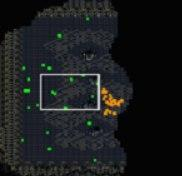
\includegraphics[width=.22\textwidth]{figures/spreading_behaviour_standard_neat}
    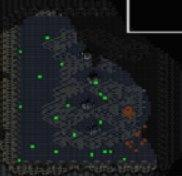
\includegraphics[width=.22\textwidth]{figures/spreading_behaviour_unified}
    \caption{Spread out behaviour with standard NEAT (left) and Unified Variant (right)}\label{fig:spreading-behaviour}
\end{figure}

In the vulture matchups, another interesting behaviour was the
vultures spreading out to cover a large area (see
Figure~\ref{fig:spreading-behaviour}) and then converge back to the
enemy once it's spotted.

However, this behaviour tends to disappear like the stimpack behaviour,
probably because the fitness of these individuals is not as good for
various reasons.  It may be because spreading out and converging back
takes time and lead to less damages inflicted or because some
individuals which had the spreading behaviour without attacking
afterward, especially for the Unified Variant where the behaviour is
often lost very quickly when not even a single unit tries to attack.
Moreover, we didn't see the behaviour at all with Cascade-NEAT, but it
may be due to randomness.

\begin{figure}
    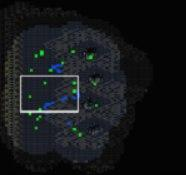
\includegraphics[width=.25\textwidth]{figures/spreading_behaviour_novelty}
    \caption{Spread out behaviour with the Novelty Variant}\label{fig:spreading-behaviour-novelty}
\end{figure}

That being said, Novelty search found a very efficient spreading
behaviour leading to a complete encirclement of the oponent as show in
Figure~\ref{fig:spreading-behaviour-novelty}.



\section{Discussion}\label{section:discussion}

TODO

Right inputs? Enough? Not Enough? (add reference to an article using interesting inputs system)

Experiments ran at full speed (not sleeping frame). I saw in an article that it has an impact on random generator quality... [FIND REF]



\section{Conclusion}\label{section:conclusion}

TODO



\section*{Acknowledgements}

AUTHOR 1 was partially funded by ACKNOWLEDGEMENT 1.

\bibliographystyle{ACM-Reference-Format}
\bibliography{bibliography}{}

\end{document}

